\documentclass{article}
\usepackage[ampersand]{easylist}
\usepackage{amsmath}
\usepackage{graphicx}
\graphicspath{ {C:/Users/ustjo/Desktop/Investing/Stocks/canslim/weeklyStockScanner/Trades/figures/} }
\usepackage[inline]{enumitem}
\usepackage{lscape}
\begin{document}
\title{Trade Summary  \\ Symbol: NVEE \\ 20180102-20180104}
\author{KAI YIN, CHAN}
\maketitle
\section{Trade details}
During 3 days holding period, price reached 51.4 cut loss point from 54.1, resulting in 49.35 realised loss.

% Table generated by Excel2LaTeX from sheet 'Sheet1'
\begin{table}[htbp]
  \centering
  \caption{Trade details}
    \begin{tabular}{p{5.145em}rrrr}
    \textbf{Date/Time} & \multicolumn{1}{p{4.215em}}{\textbf{Quantity}} & \multicolumn{1}{p{4.215em}}{\textbf{T. Price}} & \multicolumn{1}{p{4.215em}}{\textbf{Proceeds}} & \multicolumn{1}{p{4.215em}}{\textbf{Comm/Fee}} \\
    2018-01-02, 09:51:29 & 18     & 54.1 & -973.8 & -0.32 \\
    2018-01-04, 15:17:11 & -18    & 51.4   & 925.2 & -0.43 \\
    \end{tabular}%
  \label{tab:addlabel}%
\end{table}%
\section{Equity curve}
Figure \ref{Equity Curve}
\begin{figure}[h]
\caption{Equity Curve}
\label{Equity Curve}
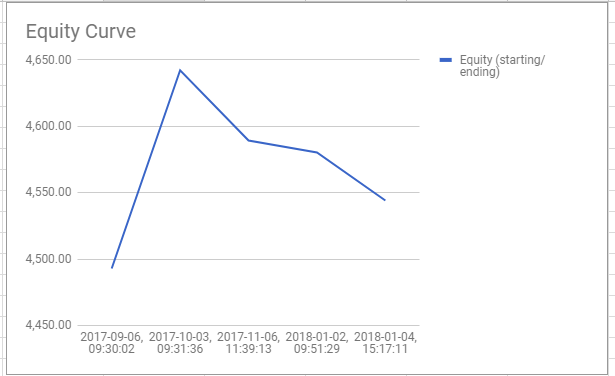
\includegraphics[width=\textwidth,keepaspectratio]{20180102-20180104_NVEE.PNG}
\end{figure}

\section{Analysis}
\subsection{Performance comparison with SPX}
Not applicable.

\iffalse
\begin{figure}
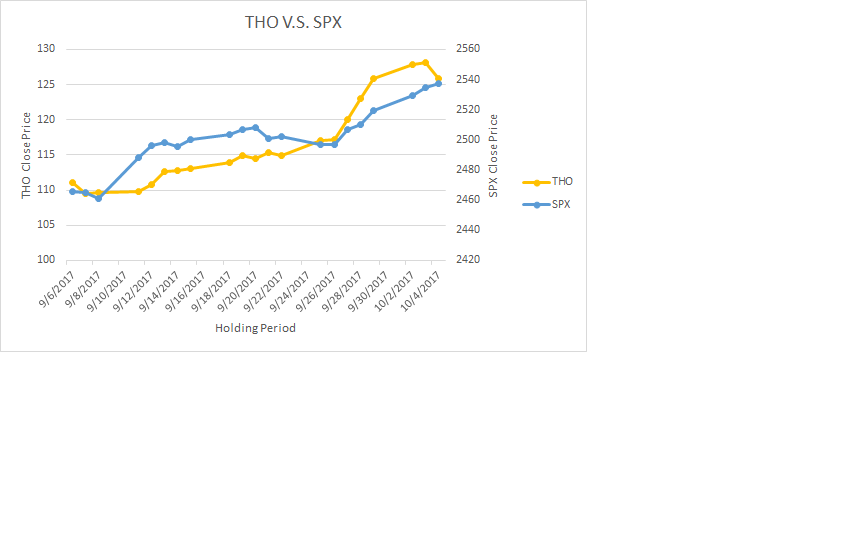
\includegraphics[width=\paperwidth,keepaspectratio] {20170906-20171003_THOSPX.PNG}
\end{figure}
\fi

\subsection{Maximum drawdown within investment period}
Not applicable.

\iffalse
\begin{figure}
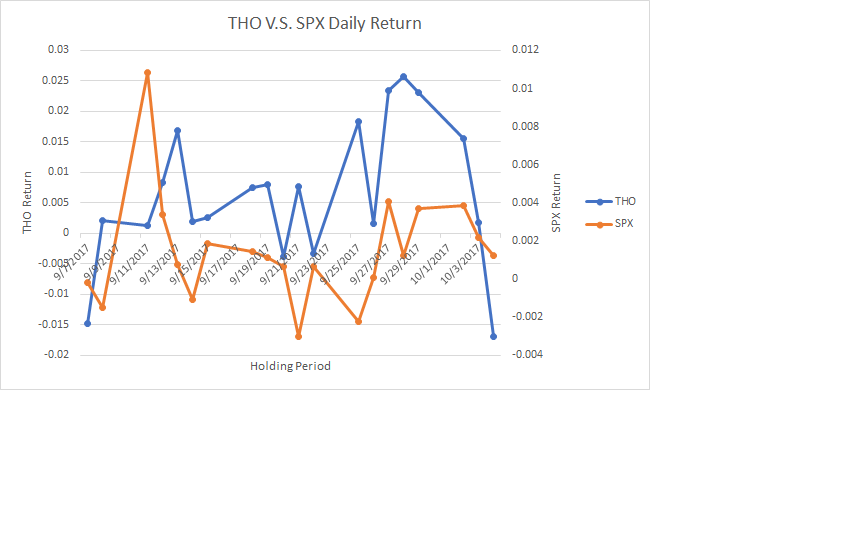
\includegraphics[width=\paperwidth,keepaspectratio]{20170906-20171003_dailyreturn.PNG}
\end{figure}
\fi

\section{Reflection}
The reason why I had chosen NVEE was a double bottom patter (Figure \ref{double bottom}). But I overlooked that I need to wait for a spike in volume in order to confirm a breakout. After checking the stock scanner document which details my trading strategy, I have missed the section about breakout. Clearly, I did not put enough attention to this.

\begin{figure}[h]
	\caption{double bottom}
	\label{double bottom}
	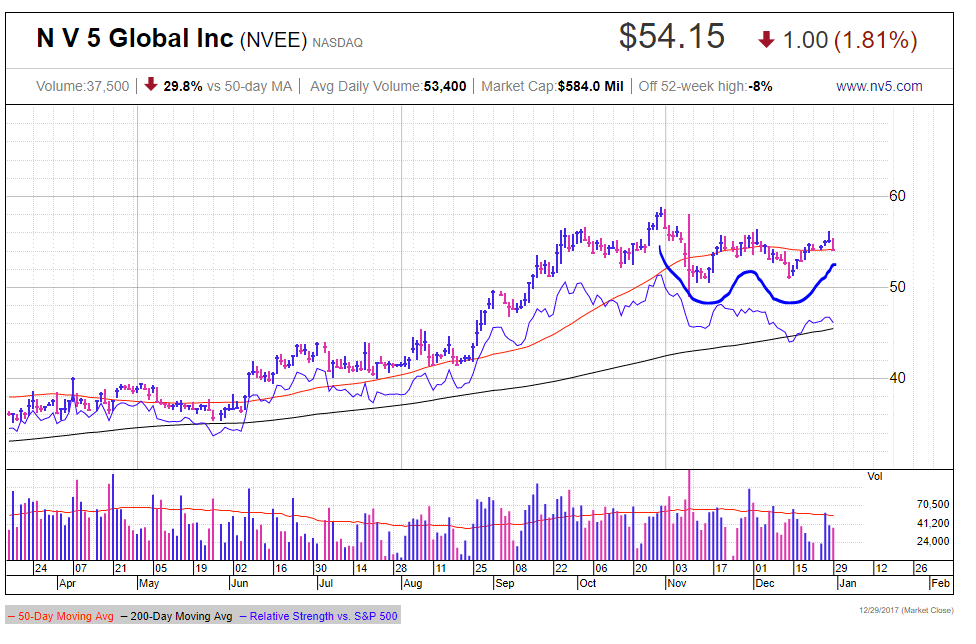
\includegraphics[width=\linewidth, keepaspectratio]{NVEE_20180101.PNG}
\end{figure}
\end{document}
